\chapter{Implementation}
\section{Foreword}
This section serves as engineering documentation for the project. All data models in the codebase are thoroughly decorated with in-editor documentation using \texttt{JsDoc}. React's tree structure also naturally guides new contributors through the app's component hierarchy, and thus this chapter focuses on rationalising the design and infrastructure choices made throughout the project. A working familiarity with a few technologies is implicitly assumed:

\begin{itemize}
    \item Source and version control (Github)
    \item Front-end web development: HTML, CSS and Javascript
    \item Back-ends, databases and remote cloud services
\end{itemize}

For the sake of brevity, sections will contain links to documentation pages of relevant libraries. Since they are not academic references, documentation of relevant libraries will be referenced using footnotes or in-text links, which further facilitate easy, immediate reference.

The goal is to create a high-quality app platform that is built for legacy and continued work. The first step is therefore to implement previously non-existent development infrastructure, especially since the online nature of the new app involves secret keys which can be monetarily exploited if compromised.

\section{DevOps Focus}
Developers often break their own code. Facebook, one of the world's largest social media giants, is known for the quality of their engineers. Yet, one of their key tenets is ``Move fast, break things'', for fear of causing a malfunction in code is one of the largest inhibitors of progress. Yet, system downtime and app crashes often shake customer confidence in a product. \href{https://aws.amazon.com/devops/what-is-devops/}{DevOps}, as it is now known in the industry, is a set of practices dedicated to speeding up code delivery by ensuring that faulty code never reaches customers, while allowing developers to iterate and experiment behind the scenes.

The following sections outline the focal points of the infrastructure and tooling choices made in this project from a DevOps engineer's perspective.

\subsection{Developer Workflow}
The code is currently hosted open-source on \href{https://github.com/Darrekt/within-react-native}{Github}. Github offers many features which facilitate the implementation of many popular DevOps practices. A few examples are listed below, and will be elaborated on in further sections.

\begin{itemize}
    \item Secret keys are stored in non-readable repository secrets.
    \item Non-collaborators cannot push changes directly to the repository.
    \item Changes cannot be pushed to the \texttt{main} branch without all tests passing and an approving review from an approved author, who cannot be the one who submitted the pull request.
    \item The build on the \texttt{main} branch is automatically deployed as the latest release whenever a change is effected.
\end{itemize}

In order to correctly maximise the utility of these features, a developer workflow is outlined in the project \texttt{README}. Invited collaborators may clone the repository directly and develop features on a separate branch, which will be merged into a staging branch (\texttt{development-staging}) before being approved to \texttt{main}. Non-collaborators who wish to contribute may fork the repository and submit a pull request from their fork, as per open-source norms.

\subsection{Continuous Integration / Continuous Deployment}
Continuous integration and deployment (or CI/CD) for short, is one of the cornerstones of DevOps. It automates and streamlines the development process in a way that allows developers to focus on business requirements and code quality instead of tedious deployment processes. Human error in the deployment process is also often the cause of system-wide failures and compromise of secret information, further motivating tested automation.

Often, this is achieved by commissioning remote machines to run scripted actions (often called ``jobs'') whenever the codebase is updated. For this reason, many CI/CD solutions are offered as add-ons or plugins to popular version control systems. This section documents the jobs which implement the CI/CD pipeline for this project. All jobs are implemented with Github Actions under the \texttt{.github/workflows} folder in the root of the project repository.

Github actions provide unlimited minutes to open-source repositories. Currently, the jobs take a total of about 20 minutes on each code change, which would easily exceed the quota for a private repository. If the code is to go closed-source for any reason, it may therefore be of interest to change to an alternate solution such as Travis CI or CircleCI.

\subsection{Regression Testing and Runtime Stability}
A key tenet of the software development lifecycle is to test code before deploying it. To this end, this project uses the open-source Jest testing library by Facebook. Jest implements a configurable test suite which recursively searches an entire Javascript project directory for any files ending in the \texttt{.test.js} extension, and provides a declarative syntax for writing and running tests. Developers can simply test for code regression by running a single command, and Jest displays a full breakdown of any test that failed as a result of recent code changes. The test suite is automatically run with every commit the main, android and ios branches of the repository, and will cause the jobs running them to produce an error whenever the test suite fails.

Additionally, Javascript as a language is dynamically typed and thus highly prone to runtime errors. This, along with the use of React.JS's rendering engine, motivate the use of Typescript and immutable data. we will later see examples of how using strongly type-checked immutable data structures to track the state of the app greatly reduces the occurence of runtime errors that would have otherwise have been very difficult to detect using vanilla React.JS.

\subsection{Build Stability}

\begin{figure}[h]
    \begin{center}
        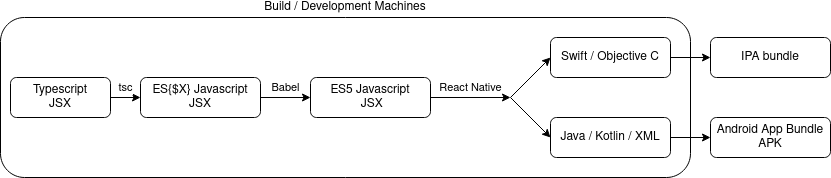
\includegraphics[scale=0.55]{images/app_build_path.png}
    \end{center}
    \caption{An example of the application build process.}
    \label{fig:app_build_process}
\end{figure}

By nature, React Native transpiles a React-like JavaScript codebase into an Android Kotlin project or an iOS project in Objective C. Figure \ref{fig:app_build_process} shows the build process of the toolchain involved in this application. Each step in the build process in this case involves a source-to-source compiler, which has to bridge semantic equivalents and substitutes between languages and frameworks. As these compilers are all open source, they, along with their many dependencies, are constantly changing.

Throughout the development of this project, there were many instances in which the project would suddenly fail to build on Android or iOS after a period of development downtime without any change in the codebase. Most frustratingly, the project involves writing platform-specific code, which adds another dimension along which a developer could cause the project build to fail. The long toolchain involved in the project build results in enormously long stack traces, which result in a situations where a developer cannot possibly know if the project is now failing to build as a result of their own changes, or a dependency breaking along the chain. Almost every time, the cause of build failure was a version dependency change in one very small library along the toolchain.

A naive solution would be to require the developer to run a script which builds app bundles for both platforms before pushing code to source control. However, building app bundles often takes a few minutes for each platform, which is extremely disruptive when developing small, rapid changes.

To address this issue, two automated jobs are defined in \texttt{android.yml} and \texttt{ios.yml}. The two jobs build the installation binaries for both native operating systems on cloud-connected build machines and throw an error if any of them fail, storing full trace logs in the job history on Github. Building the app requires the firebase configuration file, which contains secret keys and are not included in the source code. The firebase configuration files are first compressed into a tar archive, passphrase-encrypted with GPG and then uploaded to the repository root as \texttt{services.tar.gpg}. The passphrase is then kept as a repository secret, and loaded into an environment variable to decrypt and extract the configuration files on the build machine.

Developers are instantly be made aware of a build failure via email, and can immediately work on understanding if the failure was due to the most recent change, or an unexpected change in the React Native dependency chain.

\subsection{Product Deployment}
Presently, the app is not deployed on any public stores due to the release process requiring a significant investment which is outside the scope of the project. Releasing the app on either store requires a monetary investment for a developer account (USD\$125), a privacy policy hosted on an owned domain and a collection of assets for a store page listing. As a proof-of-concept and temporary workaround, the job implemented in \texttt{releasedraft.yml} automatically builds a release binary of the app whenever a change is successfully pushed to the \texttt{main} branch.

Building a release APK requires an app to be signed using a consistent set of keys as a proof-of-work from the developer. These keys are contained in a keystore, which is encoded as a base64 string and then stored as a repository secret. The decryption passphrase is similarly stored as a repository secret, and both are loaded into environment variables for decryption on the build machine. Once the app is built and signed, the resulting build artefact (the release APK) is released on the repository with a new tag. In the future, this should be updated to use the API of the respective app stores to automate the release process.

\section{Minimum Working Examples}
Minimum working examples (MWEs) are excellent ways of sanity-checking a project for feasiblity before beginning the development process. Sometimes, the explicit creation of an MWE is not necessary, as what is required is simply the knowledge that the proposed feature is possible to implement. This section thus highlights the research processes, or the resulting MWEs that were developed for some key features in the app.

\subsection{Authentication and Identity Management}
Data synchronisation is achieved through a user's unique ID, which is unified across all their logins. The secure login is implemented through the Firebase SDK, which provides a single point of unified identity management using either email credentials or one of the supported providers. In this case, the project aims to support sign ins with Google, Facebook or email. Users are able to access their data and have the same experience across devices after logging in.

While Firebase offers support for third-party login providers, these are unfortunately unavailable in the scope of this project due to the lack of presence on an app store. Apple devices require any app offering social media sign-ins to offer AppleID sign ins first, which require a verified developer account and a published app on the App Store for security reasons. However, a traditional email and password style sign-in is fully implementable.

\subsection{Do-not-disturb mode}
Preventing notifications from disturbing a user is one of the key functionalities of the app. Its previous implementation was in fact, insufficient, as some notifications could still slip through despite the user being in the middle of a work interval. The native Android SDK gives a developer the ability to invoke a callback function whenever a notification is fired by the system. The previous notification-blocking functionality thus worked by adding code within this callback to dismiss the notification. This implementation has 2 fatal flaws: firstly, the asynchronous nature of the callback invocation meant that there would be edge cases in which running tasks on the main thread would delay the dismissal of the notification, therefore firing too late to dismiss it and allowing the notification through. Secondly, the dismissal of a notification meant that a user would not see them after the work interval is complete, potentially causing the user to miss important messages or calls.

A more suitable implementation that fixes both of these faults lies in the Do-not-disturb (DnD) functionality provided by the Android OS. DnD mode suppresses notifications while active, preventing attention-grabbing features such as sound, vibration and the notification LED on the phone face. This has obvious applications for users who are driving, in important meetings, or otherwise wishing to be undisturbed. All notifications received in this mode are still visible to a user who deliberately picks up the phone and checks the notification inbox after the fact, which means users still have access to any important pieces of information delivered during the interval.

The challenge now is accessing native android APIs from within React Native. As Figure \ref{fig:app_build_process} showed previously, the entire app is written in Typescript. However, React Native offers a \texttt{NativeModules} feature which allows developers to write native code modules which may be accessed across the language gap. Full documentation is available in the \href{https://reactnative.dev/docs/native-modules-intro}{React Native guide}. From here, turning on Do-not-disturb mode programmatically is a matter of navigating the Android APIs. The full code is available in \texttt{DnDMode.java}.

\section{Structuring Productivity in Data}
\subsection{Motivation}

\subsection{Initial Data Model}
\begin{figure}[h]
    \begin{center}
        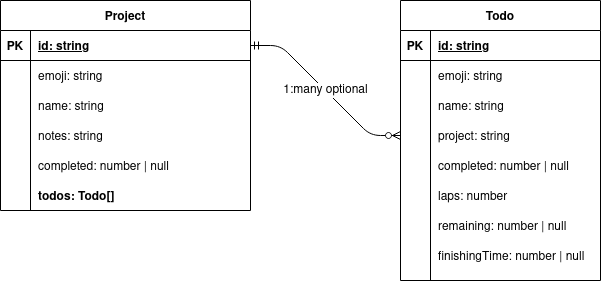
\includegraphics[scale=0.5]{images/initial_data_model.png}
    \end{center}
    \caption{The initial data model.}
    \label{fig:initial_data_model}
\end{figure}

The previous iteration of the app only had support for todos. It was decided that projects were necessary to allow users to categorise their tasks and have a specific scope of focus. Figure \ref{fig:initial_data_model} shows the Entity-relationship (ER) model to support these features. The ER model shows how the same schema might be implemented in an SQL-like database. However, noSQL stores such as Firestore often use composition to capture relationships. This is reflected in the fact that a Project contains an array of Todos, which are serialised to raw string values for storage in the database. In an SQL environment, this would be captured purely using the foreign-key relation between Projects and Todos. This replication (signified in \textbf{bold}) has been left intact, since it does not change any of the factors affecting pricing by any significant amount, and is useful in helping developers understand the relation between the two entities, should the system migrate to an SQL datastore later on.

\subsection{Revised Data Model}
\begin{figure}[h]
    \begin{center}
        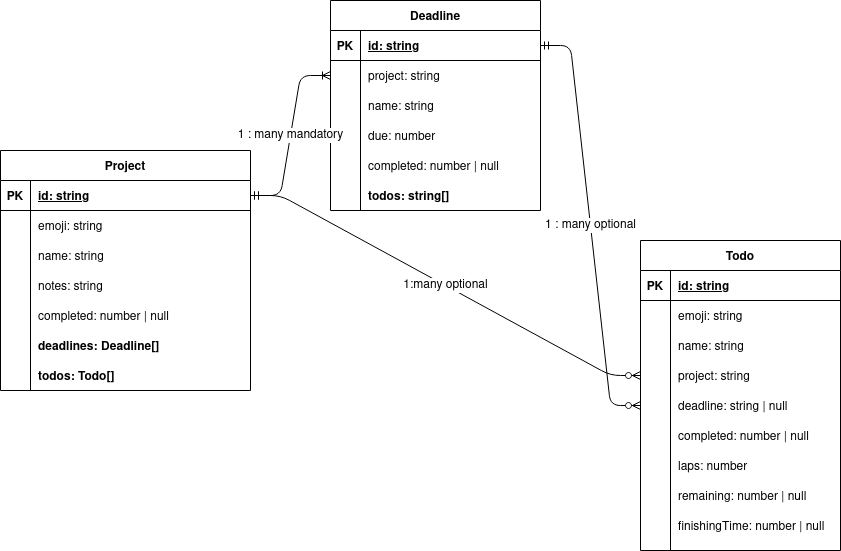
\includegraphics[scale=0.5]{images/final_data_model.png}
    \end{center}
    \caption{The current data model.}
    \label{fig:app_current_data_model}
\end{figure}

Halfway through development, it became apparent that the existing data model would not suffice to support a richer feature set. Projects needed to be broken down further into multiple deadlines, and a given deadline in focus had to be further decomposed into individual tasks on a per-session basis. Figure \ref{fig:app_current_data_model} shows the ER model for the updated schema. This model allows for a structured breakdown of complex tasks, modelled after a typical student or academic's workload.

\subsection{Syncing through snapshot listeners}
Firebase bills off of three key metrics: reads, writes and network eggress\footnote{\href{https://cloud.google.com/firestore/quotas}{Firebase quotas documentation}}. JSON-like objects are stored as documents in named collections, and documents may themselves hold subcollections. Therefore, an obvious was to optimise the schema for minimal reads is to hold more information within a single document. Reads and writes are optimised by serialising small objects into \texttt{string} representations, which can then be kept in arrays under larger entities. In Firebase, all deadlines and todos are held under a single project's document. The entire app's state is therefore encapsulated in the array of \texttt{Projects} that a given user has. Changes to any entity (Todo, Deadline or Project) also consequently only cost 1 document write under this schema.

Firebase offers snapshot listener functions as part of its Javascript API. These follow a publish / subscribe (pub/sub) model where a subscription function is passed a callback to execute. Real-time synchronisation is thus achieved by loading the updated app state into the app whenever a new state is published.

\section{User Interface}

\subsection{A brief tour of React.JS}
React.JS is a library which introduces a declarative syntax for making responsive user interfaces on the web. Readers familiar with web technologies will be familiar with the Document Object Model (DOM), which simply describes the layout of a webpage in a tree-like structure. React allows a developer to declare `what' should appear on screen, which is `rendered' as a virtual DOM. This virtual DOM is then compared with what is presently on the user's screen (the actual DOM) using a process called reconciliation, in which only the differing elements between the two trees are identified and re-rendered. This results in minimal computation to achieve the desired change in the user interface without requiring a page refresh on behalf of the user, and the result is a single-page application (SPA), which continues to be the dominant design for parts of many modern websites.

The paradigm of `thinking in React' has now become so popular that React is a dominant presence in modern web stacks, and a highly in-demand skill for developers. Reactive paradigms have been further extended to new libraries such as React Native, which has an almost identical developer experience to React.JS, but transpiles down into native code for multiple platforms.

\begin{itemize}
    \item \href{https://reactjs.org/docs/hello-world.html}{React Docs - the starting point for any React developer}
    \item \href{https://blog.isquaredsoftware.com/2020/05/blogged-answers-a-mostly-complete-guide-to-react-rendering-behavior/#rendering-process-overview}{A guide to React's rendering behaviour}
\end{itemize}

\subsection{Screen flow}